\documentclass[twoside]{book}

% Packages required by doxygen
\usepackage{fixltx2e}
\usepackage{calc}
\usepackage{doxygen}
\usepackage[export]{adjustbox} % also loads graphicx
\usepackage{graphicx}
\usepackage[utf8]{inputenc}
\usepackage{makeidx}
\usepackage{multicol}
\usepackage{multirow}
\PassOptionsToPackage{warn}{textcomp}
\usepackage{textcomp}
\usepackage[nointegrals]{wasysym}
\usepackage[table]{xcolor}

% Font selection
\usepackage[T1]{fontenc}
\usepackage[scaled=.90]{helvet}
\usepackage{courier}
\usepackage{amssymb}
\usepackage{sectsty}
\renewcommand{\familydefault}{\sfdefault}
\allsectionsfont{%
  \fontseries{bc}\selectfont%
  \color{darkgray}%
}
\renewcommand{\DoxyLabelFont}{%
  \fontseries{bc}\selectfont%
  \color{darkgray}%
}
\newcommand{\+}{\discretionary{\mbox{\scriptsize$\hookleftarrow$}}{}{}}

% Page & text layout
\usepackage{geometry}
\geometry{%
  a4paper,%
  top=2.5cm,%
  bottom=2.5cm,%
  left=2.5cm,%
  right=2.5cm%
}
\tolerance=750
\hfuzz=15pt
\hbadness=750
\setlength{\emergencystretch}{15pt}
\setlength{\parindent}{0cm}
\setlength{\parskip}{3ex plus 2ex minus 2ex}
\makeatletter
\renewcommand{\paragraph}{%
  \@startsection{paragraph}{4}{0ex}{-1.0ex}{1.0ex}{%
    \normalfont\normalsize\bfseries\SS@parafont%
  }%
}
\renewcommand{\subparagraph}{%
  \@startsection{subparagraph}{5}{0ex}{-1.0ex}{1.0ex}{%
    \normalfont\normalsize\bfseries\SS@subparafont%
  }%
}
\makeatother

% Headers & footers
\usepackage{fancyhdr}
\pagestyle{fancyplain}
\fancyhead[LE]{\fancyplain{}{\bfseries\thepage}}
\fancyhead[CE]{\fancyplain{}{}}
\fancyhead[RE]{\fancyplain{}{\bfseries\leftmark}}
\fancyhead[LO]{\fancyplain{}{\bfseries\rightmark}}
\fancyhead[CO]{\fancyplain{}{}}
\fancyhead[RO]{\fancyplain{}{\bfseries\thepage}}
\fancyfoot[LE]{\fancyplain{}{}}
\fancyfoot[CE]{\fancyplain{}{}}
\fancyfoot[RE]{\fancyplain{}{\bfseries\scriptsize Generated by Doxygen }}
\fancyfoot[LO]{\fancyplain{}{\bfseries\scriptsize Generated by Doxygen }}
\fancyfoot[CO]{\fancyplain{}{}}
\fancyfoot[RO]{\fancyplain{}{}}
\renewcommand{\footrulewidth}{0.4pt}
\renewcommand{\chaptermark}[1]{%
  \markboth{#1}{}%
}
\renewcommand{\sectionmark}[1]{%
  \markright{\thesection\ #1}%
}

% Indices & bibliography
\usepackage{natbib}
\usepackage[titles]{tocloft}
\setcounter{tocdepth}{3}
\setcounter{secnumdepth}{5}
\makeindex

% Hyperlinks (required, but should be loaded last)
\usepackage{ifpdf}
\ifpdf
  \usepackage[pdftex,pagebackref=true]{hyperref}
\else
  \usepackage[ps2pdf,pagebackref=true]{hyperref}
\fi
\hypersetup{%
  colorlinks=true,%
  linkcolor=blue,%
  citecolor=blue,%
  unicode%
}

% Custom commands
\newcommand{\clearemptydoublepage}{%
  \newpage{\pagestyle{empty}\cleardoublepage}%
}

\usepackage{caption}
\captionsetup{labelsep=space,justification=centering,font={bf},singlelinecheck=off,skip=4pt,position=top}

%===== C O N T E N T S =====

\begin{document}

% Titlepage & ToC
\hypersetup{pageanchor=false,
             bookmarksnumbered=true,
             pdfencoding=unicode
            }
\pagenumbering{alph}
\begin{titlepage}
\vspace*{7cm}
\begin{center}%
{\Large Soft\+Eng }\\
\vspace*{1cm}
{\large Generated by Doxygen 1.8.13}\\
\end{center}
\end{titlepage}
\clearemptydoublepage
\pagenumbering{roman}
\tableofcontents
\clearemptydoublepage
\pagenumbering{arabic}
\hypersetup{pageanchor=true}

%--- Begin generated contents ---
\chapter{Class Index}
\section{Class List}
Here are the classes, structs, unions and interfaces with brief descriptions\+:\begin{DoxyCompactList}
\item\contentsline{section}{\hyperlink{class_exporter}{Exporter} }{\pageref{class_exporter}}{}
\item\contentsline{section}{\hyperlink{class_exporter_c_l_i}{Exporter\+C\+LI} }{\pageref{class_exporter_c_l_i}}{}
\item\contentsline{section}{\hyperlink{class_exporter_h_t_m_l}{Exporter\+H\+T\+ML} }{\pageref{class_exporter_h_t_m_l}}{}
\item\contentsline{section}{\hyperlink{class_exporter_t_x_t}{Exporter\+T\+XT} }{\pageref{class_exporter_t_x_t}}{}
\item\contentsline{section}{\hyperlink{class_metronet}{Metronet} }{\pageref{class_metronet}}{}
\item\contentsline{section}{\hyperlink{class_parser}{Parser} }{\pageref{class_parser}}{}
\item\contentsline{section}{\hyperlink{class_spoor}{Spoor} }{\pageref{class_spoor}}{}
\item\contentsline{section}{\hyperlink{class_station}{Station} }{\pageref{class_station}}{}
\item\contentsline{section}{\hyperlink{class_tram}{Tram} }{\pageref{class_tram}}{}
\end{DoxyCompactList}

\chapter{Class Documentation}
\hypertarget{class_exporter}{}\section{Exporter Class Reference}
\label{class_exporter}\index{Exporter@{Exporter}}


\hyperlink{class_exporter}{Exporter} base klasse die de output van gegevens behandelt.  




{\ttfamily \#include $<$Exporter.\+h$>$}



Inheritance diagram for Exporter\+:
\nopagebreak
\begin{figure}[H]
\begin{center}
\leavevmode
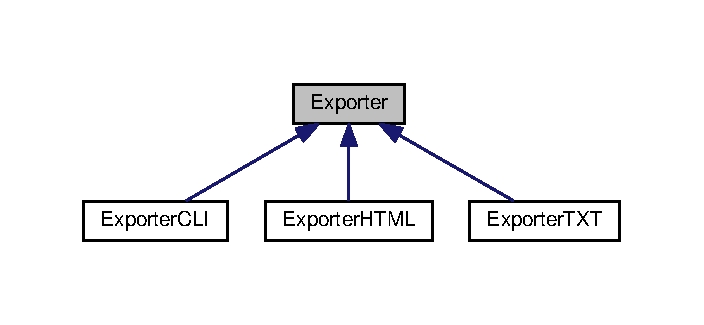
\includegraphics[width=350pt]{class_exporter__inherit__graph}
\end{center}
\end{figure}


Collaboration diagram for Exporter\+:
\nopagebreak
\begin{figure}[H]
\begin{center}
\leavevmode
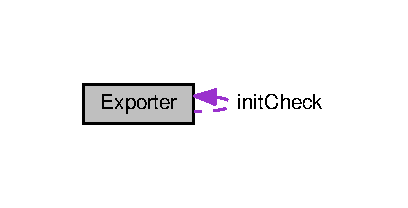
\includegraphics[width=204pt]{class_exporter__coll__graph}
\end{center}
\end{figure}
\subsection*{Public Member Functions}
\begin{DoxyCompactItemize}
\item 
\hyperlink{class_exporter_a2a977cb5ac8f637fcb570e73f650eca0}{Exporter} ()
\begin{DoxyCompactList}\small\item\em Lege constructor van \hyperlink{class_exporter}{Exporter}. \end{DoxyCompactList}\item 
bool \hyperlink{class_exporter_afba4e69e23ad018c26b21c0f4b85ef12}{is\+Document\+Started} () const 
\begin{DoxyCompactList}\small\item\em Getter van member document\+Started. \end{DoxyCompactList}\item 
virtual bool \hyperlink{class_exporter_af01d2a6c2f54329b1867a19537e11a34}{properly\+Initialised} () const 
\begin{DoxyCompactList}\small\item\em Kijk na of de constructor in de juiste staat geeindigd is. \end{DoxyCompactList}\item 
virtual void \hyperlink{class_exporter_ab3736803133eb727cf87a7306f91eb11}{write} (std\+::string \&output, std\+::ostream \&os)
\begin{DoxyCompactList}\small\item\em Stuur de output string naar de output stream. \end{DoxyCompactList}\item 
virtual void \hyperlink{class_exporter_ae477714f462d70cfc5b3970f91fcc4ed}{finish} (std\+::ostream \&os)
\begin{DoxyCompactList}\small\item\em Stuurt de nodige informatie naar de output stream om het document correct af te sluiten. \end{DoxyCompactList}\end{DoxyCompactItemize}
\subsection*{Protected Attributes}
\begin{DoxyCompactItemize}
\item 
bool \hyperlink{class_exporter_a7d55f6023d5fe983512f6b02fb60733b}{document\+Started}
\item 
\hyperlink{class_exporter}{Exporter} $\ast$ \hyperlink{class_exporter_a74245e988d8e72a43704dda927acff05}{init\+Check}
\end{DoxyCompactItemize}


\subsection{Detailed Description}
\hyperlink{class_exporter}{Exporter} base klasse die de output van gegevens behandelt. 

\subsection{Constructor \& Destructor Documentation}
\index{Exporter@{Exporter}!Exporter@{Exporter}}
\index{Exporter@{Exporter}!Exporter@{Exporter}}
\subsubsection[{\texorpdfstring{Exporter()}{Exporter()}}]{\setlength{\rightskip}{0pt plus 5cm}Exporter\+::\+Exporter (
\begin{DoxyParamCaption}
{}
\end{DoxyParamCaption}
)}\hypertarget{class_exporter_a2a977cb5ac8f637fcb570e73f650eca0}{}\label{class_exporter_a2a977cb5ac8f637fcb570e73f650eca0}


Lege constructor van \hyperlink{class_exporter}{Exporter}. 



\subsection{Member Function Documentation}
\index{Exporter@{Exporter}!finish@{finish}}
\index{finish@{finish}!Exporter@{Exporter}}
\subsubsection[{\texorpdfstring{finish(std\+::ostream \&os)}{finish(std::ostream &os)}}]{\setlength{\rightskip}{0pt plus 5cm}void Exporter\+::finish (
\begin{DoxyParamCaption}
\item[{std\+::ostream \&}]{os}
\end{DoxyParamCaption}
)\hspace{0.3cm}{\ttfamily [virtual]}}\hypertarget{class_exporter_ae477714f462d70cfc5b3970f91fcc4ed}{}\label{class_exporter_ae477714f462d70cfc5b3970f91fcc4ed}


Stuurt de nodige informatie naar de output stream om het document correct af te sluiten. 


\begin{DoxyParams}{Parameters}
{\em os} & De stream waar de output naar gestuurd zal worden. \\
\hline
\end{DoxyParams}
\begin{DoxyPrecond}{Precondition}
R\+E\+Q\+U\+I\+RE(this-\/$>$\hyperlink{class_exporter_af01d2a6c2f54329b1867a19537e11a34}{properly\+Initialised()}, \char`\"{}\+Exporter was niet geinitialiseerd bij de aanroep van finish.\char`\"{}); 

R\+E\+Q\+U\+I\+RE(document\+Started, \char`\"{}\+Document was niet aangemaakt voor de aanroep van finish.\char`\"{}); 
\end{DoxyPrecond}


Reimplemented in \hyperlink{class_exporter_h_t_m_l_aefa1c658f3c3c55bd7725bdad09629b3}{Exporter\+H\+T\+ML}.



Here is the call graph for this function\+:
\nopagebreak
\begin{figure}[H]
\begin{center}
\leavevmode
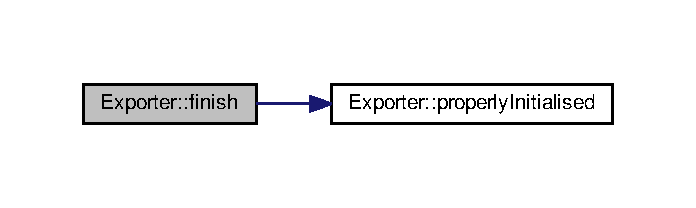
\includegraphics[width=350pt]{class_exporter_ae477714f462d70cfc5b3970f91fcc4ed_cgraph}
\end{center}
\end{figure}




Here is the caller graph for this function\+:
\nopagebreak
\begin{figure}[H]
\begin{center}
\leavevmode
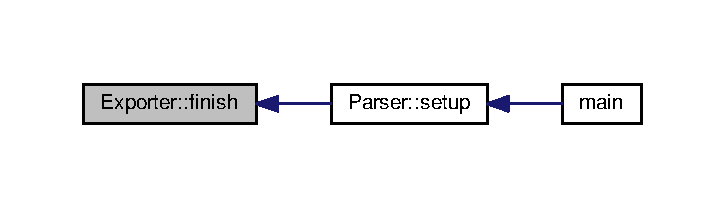
\includegraphics[width=263pt]{class_exporter_ae477714f462d70cfc5b3970f91fcc4ed_icgraph}
\end{center}
\end{figure}


\index{Exporter@{Exporter}!is\+Document\+Started@{is\+Document\+Started}}
\index{is\+Document\+Started@{is\+Document\+Started}!Exporter@{Exporter}}
\subsubsection[{\texorpdfstring{is\+Document\+Started() const }{isDocumentStarted() const }}]{\setlength{\rightskip}{0pt plus 5cm}bool Exporter\+::is\+Document\+Started (
\begin{DoxyParamCaption}
{}
\end{DoxyParamCaption}
) const}\hypertarget{class_exporter_afba4e69e23ad018c26b21c0f4b85ef12}{}\label{class_exporter_afba4e69e23ad018c26b21c0f4b85ef12}


Getter van member document\+Started. 

\begin{DoxyReturn}{Returns}
De waarde van document\+Started 
\end{DoxyReturn}
\begin{DoxyPrecond}{Precondition}
R\+E\+Q\+U\+I\+RE(this-\/$>$\hyperlink{class_exporter_af01d2a6c2f54329b1867a19537e11a34}{properly\+Initialised()}, \char`\"{}\+Exporter was niet geinitialiseerd bij de aanroep van is\+Document\+Started.\char`\"{}); 
\end{DoxyPrecond}


Here is the call graph for this function\+:
\nopagebreak
\begin{figure}[H]
\begin{center}
\leavevmode
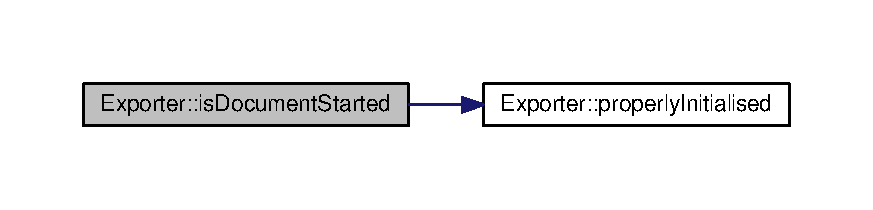
\includegraphics[width=350pt]{class_exporter_afba4e69e23ad018c26b21c0f4b85ef12_cgraph}
\end{center}
\end{figure}




Here is the caller graph for this function\+:
\nopagebreak
\begin{figure}[H]
\begin{center}
\leavevmode
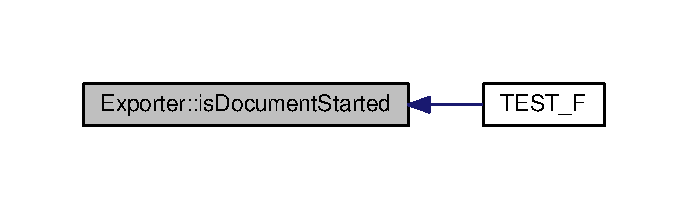
\includegraphics[width=330pt]{class_exporter_afba4e69e23ad018c26b21c0f4b85ef12_icgraph}
\end{center}
\end{figure}


\index{Exporter@{Exporter}!properly\+Initialised@{properly\+Initialised}}
\index{properly\+Initialised@{properly\+Initialised}!Exporter@{Exporter}}
\subsubsection[{\texorpdfstring{properly\+Initialised() const }{properlyInitialised() const }}]{\setlength{\rightskip}{0pt plus 5cm}bool Exporter\+::properly\+Initialised (
\begin{DoxyParamCaption}
{}
\end{DoxyParamCaption}
) const\hspace{0.3cm}{\ttfamily [virtual]}}\hypertarget{class_exporter_af01d2a6c2f54329b1867a19537e11a34}{}\label{class_exporter_af01d2a6c2f54329b1867a19537e11a34}


Kijk na of de constructor in de juiste staat geeindigd is. 

\begin{DoxyReturn}{Returns}
Boolean die aangeeft of het object juist geinitialiseerd is. 
\end{DoxyReturn}


Here is the caller graph for this function\+:
\nopagebreak
\begin{figure}[H]
\begin{center}
\leavevmode
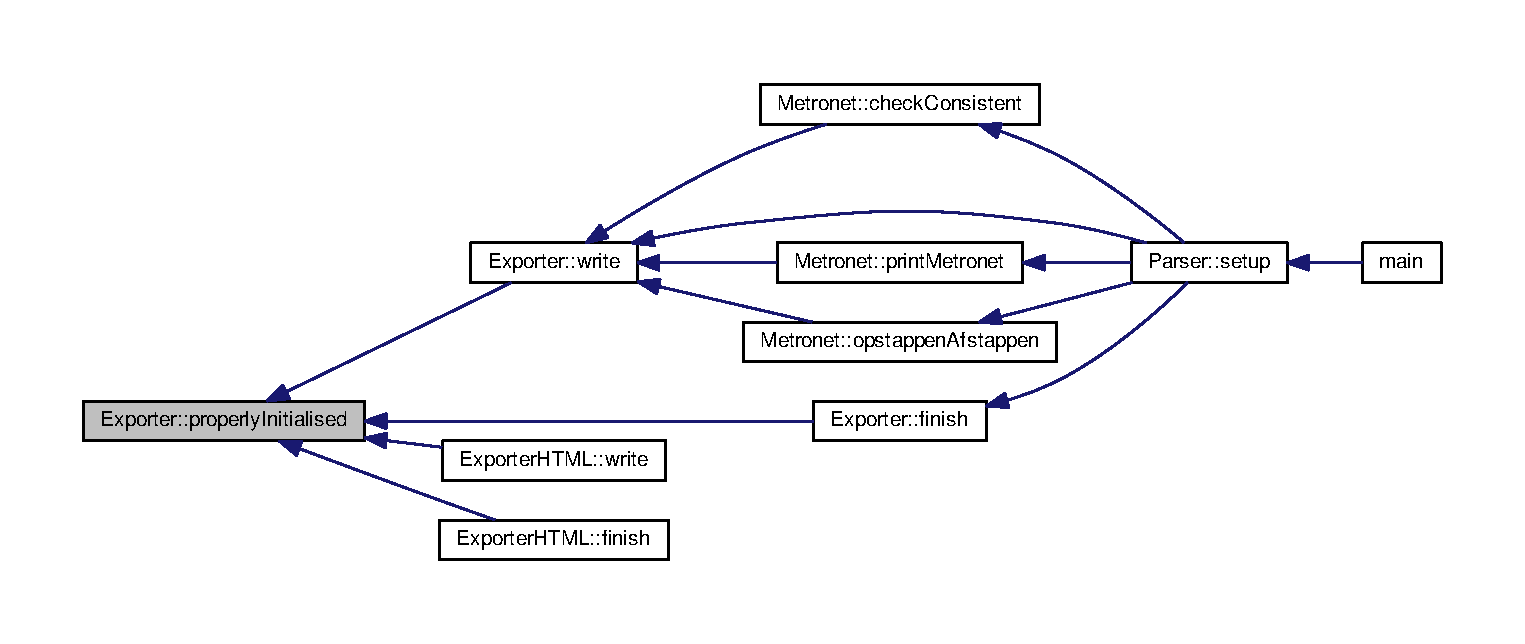
\includegraphics[width=350pt]{class_exporter_af01d2a6c2f54329b1867a19537e11a34_icgraph}
\end{center}
\end{figure}


\index{Exporter@{Exporter}!write@{write}}
\index{write@{write}!Exporter@{Exporter}}
\subsubsection[{\texorpdfstring{write(std\+::string \&output, std\+::ostream \&os)}{write(std::string &output, std::ostream &os)}}]{\setlength{\rightskip}{0pt plus 5cm}void Exporter\+::write (
\begin{DoxyParamCaption}
\item[{std\+::string \&}]{output, }
\item[{std\+::ostream \&}]{os}
\end{DoxyParamCaption}
)\hspace{0.3cm}{\ttfamily [virtual]}}\hypertarget{class_exporter_ab3736803133eb727cf87a7306f91eb11}{}\label{class_exporter_ab3736803133eb727cf87a7306f91eb11}


Stuur de output string naar de output stream. 


\begin{DoxyParams}{Parameters}
{\em output} & De string die naar de output gestuurd moet worden. \\
\hline
{\em os} & De stream waar de output naar gestuurd zal worden. \\
\hline
\end{DoxyParams}
\begin{DoxyPrecond}{Precondition}
R\+E\+Q\+U\+I\+RE(this-\/$>$\hyperlink{class_exporter_af01d2a6c2f54329b1867a19537e11a34}{properly\+Initialised()}, \char`\"{}\+Exporter was niet geinitialiseerd bij de aanroep van write.\char`\"{}); 
\end{DoxyPrecond}
\begin{DoxyPostcond}{Postcondition}
E\+N\+S\+U\+RE(document\+Started, \char`\"{}\+Document was niet aangemaakt bij de aanroep van write.\char`\"{}); 
\end{DoxyPostcond}


Reimplemented in \hyperlink{class_exporter_h_t_m_l_ace2649c240282289d4cb3bfbd19e427c}{Exporter\+H\+T\+ML}.



Here is the call graph for this function\+:
\nopagebreak
\begin{figure}[H]
\begin{center}
\leavevmode
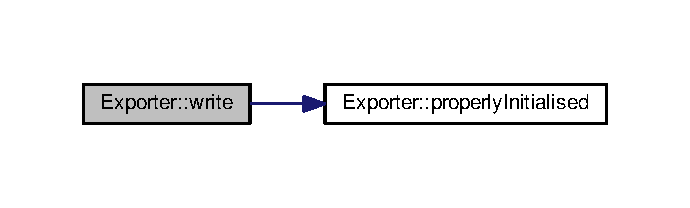
\includegraphics[width=350pt]{class_exporter_ab3736803133eb727cf87a7306f91eb11_cgraph}
\end{center}
\end{figure}




Here is the caller graph for this function\+:
\nopagebreak
\begin{figure}[H]
\begin{center}
\leavevmode
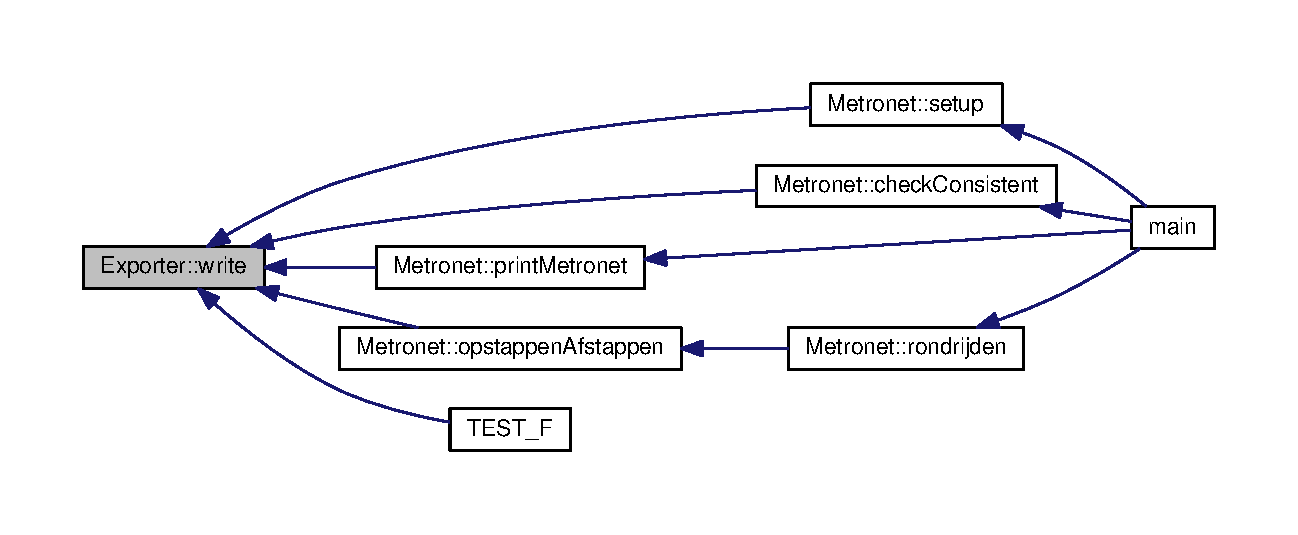
\includegraphics[width=350pt]{class_exporter_ab3736803133eb727cf87a7306f91eb11_icgraph}
\end{center}
\end{figure}




\subsection{Member Data Documentation}
\index{Exporter@{Exporter}!document\+Started@{document\+Started}}
\index{document\+Started@{document\+Started}!Exporter@{Exporter}}
\subsubsection[{\texorpdfstring{document\+Started}{documentStarted}}]{\setlength{\rightskip}{0pt plus 5cm}bool Exporter\+::document\+Started\hspace{0.3cm}{\ttfamily [protected]}}\hypertarget{class_exporter_a7d55f6023d5fe983512f6b02fb60733b}{}\label{class_exporter_a7d55f6023d5fe983512f6b02fb60733b}
\index{Exporter@{Exporter}!init\+Check@{init\+Check}}
\index{init\+Check@{init\+Check}!Exporter@{Exporter}}
\subsubsection[{\texorpdfstring{init\+Check}{initCheck}}]{\setlength{\rightskip}{0pt plus 5cm}{\bf Exporter}$\ast$ Exporter\+::init\+Check\hspace{0.3cm}{\ttfamily [protected]}}\hypertarget{class_exporter_a74245e988d8e72a43704dda927acff05}{}\label{class_exporter_a74245e988d8e72a43704dda927acff05}


The documentation for this class was generated from the following files\+:\begin{DoxyCompactItemize}
\item 
/home/jonathan/\+Desktop/\+Project Software Engineering/\+Metronet/\+P\+S\+E/src/\hyperlink{_exporter_8h}{Exporter.\+h}\item 
/home/jonathan/\+Desktop/\+Project Software Engineering/\+Metronet/\+P\+S\+E/src/\hyperlink{_exporter_8cpp}{Exporter.\+cpp}\end{DoxyCompactItemize}

\hypertarget{class_metronet}{}\section{Metronet Class Reference}
\label{class_metronet}\index{Metronet@{Metronet}}
\subsection*{Public Member Functions}
\begin{DoxyCompactItemize}
\item 
\mbox{\Hypertarget{class_metronet_a3d2adce29a947f162924279b766de645}\label{class_metronet_a3d2adce29a947f162924279b766de645}} 
bool \hyperlink{class_metronet_a3d2adce29a947f162924279b766de645}{properly\+Initialised} ()
\begin{DoxyCompactList}\small\item\em Kijk na of de constructor in de juiste staat geeindigd is. \end{DoxyCompactList}\item 
void \hyperlink{class_metronet_a37106294bf52324b0fb9fcecf11e5495}{add\+Station} (\hyperlink{class_station}{Station} $\ast$)
\begin{DoxyCompactList}\small\item\em Voegt station toe aan metronet. \end{DoxyCompactList}\item 
void \hyperlink{class_metronet_ab9bcc898b7b0ec5571ce149364cf64fc}{add\+Tram} (\hyperlink{class_tram}{Tram} $\ast$)
\begin{DoxyCompactList}\small\item\em Voegt tram toe aan metronet. \end{DoxyCompactList}\item 
void \hyperlink{class_metronet_ab6faa9e35828352e4003640d13798529}{add\+Spoor} (\hyperlink{class_spoor}{Spoor} $\ast$)
\begin{DoxyCompactList}\small\item\em Voegt spoor toe aan metronet. \end{DoxyCompactList}\item 
bool \hyperlink{class_metronet_a0128de167ec0a36e70abd57170b3faed}{check\+Consistent} (\hyperlink{class_exporter}{Exporter} $\ast$exp)
\begin{DoxyCompactList}\small\item\em Kijkt na of het metronet consistent is. \end{DoxyCompactList}\end{DoxyCompactItemize}


\subsection{Member Function Documentation}
\mbox{\Hypertarget{class_metronet_ab6faa9e35828352e4003640d13798529}\label{class_metronet_ab6faa9e35828352e4003640d13798529}} 
\index{Metronet@{Metronet}!add\+Spoor@{add\+Spoor}}
\index{add\+Spoor@{add\+Spoor}!Metronet@{Metronet}}
\subsubsection{\texorpdfstring{add\+Spoor()}{addSpoor()}}
{\footnotesize\ttfamily void Metronet\+::add\+Spoor (\begin{DoxyParamCaption}\item[{\hyperlink{class_spoor}{Spoor} $\ast$}]{spoor }\end{DoxyParamCaption})}



Voegt spoor toe aan metronet. 

R\+E\+Q\+U\+I\+RE(this-\/$>$\hyperlink{class_metronet_a3d2adce29a947f162924279b766de645}{properly\+Initialised()}, \char`\"{}\+Metronet was niet geinitialiseerd bij de aanroep van add\+Spoor.\char`\"{});~\newline
R\+E\+Q\+U\+I\+RE(Spoor-\/$>$\hyperlink{class_metronet_a3d2adce29a947f162924279b766de645}{properly\+Initialised()}, \char`\"{}\+Spoor was niet geinitialiseerd bij de aanroep van add\+Spoor.\char`\"{});~\newline
E\+N\+S\+U\+RE(sporen\mbox{[}sporen.\+size() -\/ 1\mbox{]} == \hyperlink{class_spoor}{Spoor}), \char`\"{}\+Spoor was niet toegevoegd bij de aanroep van add\+Spoor.\char`\"{});~\newline
\mbox{\Hypertarget{class_metronet_a37106294bf52324b0fb9fcecf11e5495}\label{class_metronet_a37106294bf52324b0fb9fcecf11e5495}} 
\index{Metronet@{Metronet}!add\+Station@{add\+Station}}
\index{add\+Station@{add\+Station}!Metronet@{Metronet}}
\subsubsection{\texorpdfstring{add\+Station()}{addStation()}}
{\footnotesize\ttfamily void Metronet\+::add\+Station (\begin{DoxyParamCaption}\item[{\hyperlink{class_station}{Station} $\ast$}]{station }\end{DoxyParamCaption})}



Voegt station toe aan metronet. 

R\+E\+Q\+U\+I\+RE(this-\/$>$\hyperlink{class_metronet_a3d2adce29a947f162924279b766de645}{properly\+Initialised()}, \char`\"{}\+Metronet was niet geinitialiseerd bij de aanroep van add\+Station.\char`\"{});~\newline
R\+E\+Q\+U\+I\+RE(Station-\/$>$\hyperlink{class_metronet_a3d2adce29a947f162924279b766de645}{properly\+Initialised()}, \char`\"{}\+Station was niet geinitialiseerd bij de aanroep van add\+Station.\char`\"{});~\newline
E\+N\+S\+U\+RE(stations\mbox{[}stations.\+size() -\/ 1\mbox{]} == \hyperlink{class_station}{Station}), \char`\"{}\+Station was niet toegevoegd bij de aanroep van add\+Station.\char`\"{});~\newline
\mbox{\Hypertarget{class_metronet_ab9bcc898b7b0ec5571ce149364cf64fc}\label{class_metronet_ab9bcc898b7b0ec5571ce149364cf64fc}} 
\index{Metronet@{Metronet}!add\+Tram@{add\+Tram}}
\index{add\+Tram@{add\+Tram}!Metronet@{Metronet}}
\subsubsection{\texorpdfstring{add\+Tram()}{addTram()}}
{\footnotesize\ttfamily void Metronet\+::add\+Tram (\begin{DoxyParamCaption}\item[{\hyperlink{class_tram}{Tram} $\ast$}]{tram }\end{DoxyParamCaption})}



Voegt tram toe aan metronet. 

R\+E\+Q\+U\+I\+RE(this-\/$>$\hyperlink{class_metronet_a3d2adce29a947f162924279b766de645}{properly\+Initialised()}, \char`\"{}\+Metronet was niet geinitialiseerd bij de aanroep van add\+Tram.\char`\"{});~\newline
R\+E\+Q\+U\+I\+RE(Tram-\/$>$\hyperlink{class_metronet_a3d2adce29a947f162924279b766de645}{properly\+Initialised()}, \char`\"{}\+Tram was niet geinitialiseerd bij de aanroep van add\+Tram.\char`\"{});~\newline
E\+N\+S\+U\+RE(trams\mbox{[}trams.\+size() -\/ 1\mbox{]} == \hyperlink{class_tram}{Tram}), \char`\"{}\+Tram was niet toegevoegd bij de aanroep van add\+Tram.\char`\"{});~\newline
\mbox{\Hypertarget{class_metronet_a0128de167ec0a36e70abd57170b3faed}\label{class_metronet_a0128de167ec0a36e70abd57170b3faed}} 
\index{Metronet@{Metronet}!check\+Consistent@{check\+Consistent}}
\index{check\+Consistent@{check\+Consistent}!Metronet@{Metronet}}
\subsubsection{\texorpdfstring{check\+Consistent()}{checkConsistent()}}
{\footnotesize\ttfamily bool Metronet\+::check\+Consistent (\begin{DoxyParamCaption}\item[{\hyperlink{class_exporter}{Exporter} $\ast$}]{exp }\end{DoxyParamCaption})}



Kijkt na of het metronet consistent is. 


\begin{DoxyParams}{Parameters}
{\em exp} & De exporter die de output zal behandelen. R\+E\+Q\+U\+I\+RE(this-\/$>$\hyperlink{class_metronet_a3d2adce29a947f162924279b766de645}{properly\+Initialised()}, \char`\"{}\+Metronet was niet geinitialiseerd bij de aanroep van check\+Consistent.\char`\"{});~\newline
\\
\hline
\end{DoxyParams}


The documentation for this class was generated from the following files\+:\begin{DoxyCompactItemize}
\item 
/home/sergio/\+C\+Lion\+Projects/\+Soft\+Eng/src/Metronet.\+h\item 
/home/sergio/\+C\+Lion\+Projects/\+Soft\+Eng/src/Metronet.\+cpp\end{DoxyCompactItemize}

\hypertarget{class_parser}{}\section{Parser Class Reference}
\label{class_parser}\index{Parser@{Parser}}


{\ttfamily \#include $<$Parser.\+h$>$}

\subsection*{Public Member Functions}
\begin{DoxyCompactItemize}
\item 
\hyperlink{class_parser_a12234f6cd36b61af4b50c94a179422c1}{Parser} ()
\item 
virtual \hyperlink{class_parser_a3e658b5917a93a3ef648050d060e3a93}{$\sim$\+Parser} ()
\end{DoxyCompactItemize}


\subsection{Constructor \& Destructor Documentation}
\mbox{\Hypertarget{class_parser_a12234f6cd36b61af4b50c94a179422c1}\label{class_parser_a12234f6cd36b61af4b50c94a179422c1}} 
\index{Parser@{Parser}!Parser@{Parser}}
\index{Parser@{Parser}!Parser@{Parser}}
\subsubsection{\texorpdfstring{Parser()}{Parser()}}
{\footnotesize\ttfamily Parser\+::\+Parser (\begin{DoxyParamCaption}{ }\end{DoxyParamCaption})}

\mbox{\Hypertarget{class_parser_a3e658b5917a93a3ef648050d060e3a93}\label{class_parser_a3e658b5917a93a3ef648050d060e3a93}} 
\index{Parser@{Parser}!````~Parser@{$\sim$\+Parser}}
\index{````~Parser@{$\sim$\+Parser}!Parser@{Parser}}
\subsubsection{\texorpdfstring{$\sim$\+Parser()}{~Parser()}}
{\footnotesize\ttfamily Parser\+::$\sim$\+Parser (\begin{DoxyParamCaption}{ }\end{DoxyParamCaption})\hspace{0.3cm}{\ttfamily [virtual]}}



The documentation for this class was generated from the following files\+:\begin{DoxyCompactItemize}
\item 
/home/sergio/\+Eclipse\+Projects/\+Soft\+Eng/src/\hyperlink{_parser_8h}{Parser.\+h}\item 
/home/sergio/\+Eclipse\+Projects/\+Soft\+Eng/src/\hyperlink{_parser_8cpp}{Parser.\+cpp}\end{DoxyCompactItemize}

\hypertarget{class_spoor}{}\section{Spoor Class Reference}
\label{class_spoor}\index{Spoor@{Spoor}}


{\ttfamily \#include $<$Spoor.\+h$>$}

\subsection*{Public Member Functions}
\begin{DoxyCompactItemize}
\item 
\hyperlink{class_spoor_a64778a4094d2d9cd3a08cbbef5a11787}{Spoor} ()
\item 
virtual \hyperlink{class_spoor_a58dcc52a48e4ad3ca7d9028a0065ca98}{$\sim$\+Spoor} ()
\item 
bool \hyperlink{class_spoor_a1eb7c54228676cdb7c8620104e063a3c}{properly\+Initialised} () const
\begin{DoxyCompactList}\small\item\em Kijk na of de constructor in de juiste staat geeindigd is. \end{DoxyCompactList}\item 
int \hyperlink{class_spoor_a66ebc0abcb370b1509bd7b3961a8e45a}{get\+Lijn\+Nr} () const
\begin{DoxyCompactList}\small\item\em Geef het lijn nummer terug. \end{DoxyCompactList}\end{DoxyCompactItemize}


\subsection{Constructor \& Destructor Documentation}
\mbox{\Hypertarget{class_spoor_a64778a4094d2d9cd3a08cbbef5a11787}\label{class_spoor_a64778a4094d2d9cd3a08cbbef5a11787}} 
\index{Spoor@{Spoor}!Spoor@{Spoor}}
\index{Spoor@{Spoor}!Spoor@{Spoor}}
\subsubsection{\texorpdfstring{Spoor()}{Spoor()}}
{\footnotesize\ttfamily Spoor\+::\+Spoor (\begin{DoxyParamCaption}{ }\end{DoxyParamCaption})}

\mbox{\Hypertarget{class_spoor_a58dcc52a48e4ad3ca7d9028a0065ca98}\label{class_spoor_a58dcc52a48e4ad3ca7d9028a0065ca98}} 
\index{Spoor@{Spoor}!````~Spoor@{$\sim$\+Spoor}}
\index{````~Spoor@{$\sim$\+Spoor}!Spoor@{Spoor}}
\subsubsection{\texorpdfstring{$\sim$\+Spoor()}{~Spoor()}}
{\footnotesize\ttfamily Spoor\+::$\sim$\+Spoor (\begin{DoxyParamCaption}{ }\end{DoxyParamCaption})\hspace{0.3cm}{\ttfamily [virtual]}}



\subsection{Member Function Documentation}
\mbox{\Hypertarget{class_spoor_a66ebc0abcb370b1509bd7b3961a8e45a}\label{class_spoor_a66ebc0abcb370b1509bd7b3961a8e45a}} 
\index{Spoor@{Spoor}!get\+Lijn\+Nr@{get\+Lijn\+Nr}}
\index{get\+Lijn\+Nr@{get\+Lijn\+Nr}!Spoor@{Spoor}}
\subsubsection{\texorpdfstring{get\+Lijn\+Nr()}{getLijnNr()}}
{\footnotesize\ttfamily int Spoor\+::get\+Lijn\+Nr (\begin{DoxyParamCaption}{ }\end{DoxyParamCaption}) const}



Geef het lijn nummer terug. 

\begin{DoxyReturn}{Returns}
Het aantal zitplaatsen.
\end{DoxyReturn}
R\+E\+Q\+U\+I\+RE(this-\/$>$\hyperlink{class_spoor_a1eb7c54228676cdb7c8620104e063a3c}{properly\+Initialised()}, \char`\"{}\+Spoor was niet geinitialiseerd bij de aanroep van get\+Lijn\+Nr.\char`\"{});~\newline
Here is the call graph for this function\+:\nopagebreak
\begin{figure}[H]
\begin{center}
\leavevmode
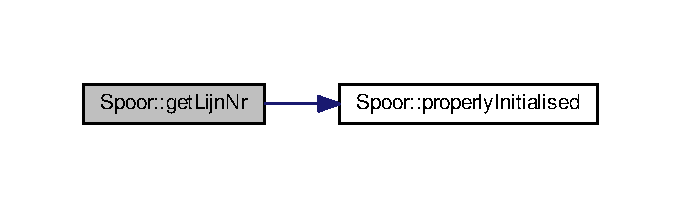
\includegraphics[width=327pt]{class_spoor_a66ebc0abcb370b1509bd7b3961a8e45a_cgraph}
\end{center}
\end{figure}
\mbox{\Hypertarget{class_spoor_a1eb7c54228676cdb7c8620104e063a3c}\label{class_spoor_a1eb7c54228676cdb7c8620104e063a3c}} 
\index{Spoor@{Spoor}!properly\+Initialised@{properly\+Initialised}}
\index{properly\+Initialised@{properly\+Initialised}!Spoor@{Spoor}}
\subsubsection{\texorpdfstring{properly\+Initialised()}{properlyInitialised()}}
{\footnotesize\ttfamily bool Spoor\+::properly\+Initialised (\begin{DoxyParamCaption}{ }\end{DoxyParamCaption}) const}



Kijk na of de constructor in de juiste staat geeindigd is. 

\begin{DoxyReturn}{Returns}
Boolean die aangeeft of het object juist geinitialiseerd is. 
\end{DoxyReturn}
Here is the caller graph for this function\+:\nopagebreak
\begin{figure}[H]
\begin{center}
\leavevmode
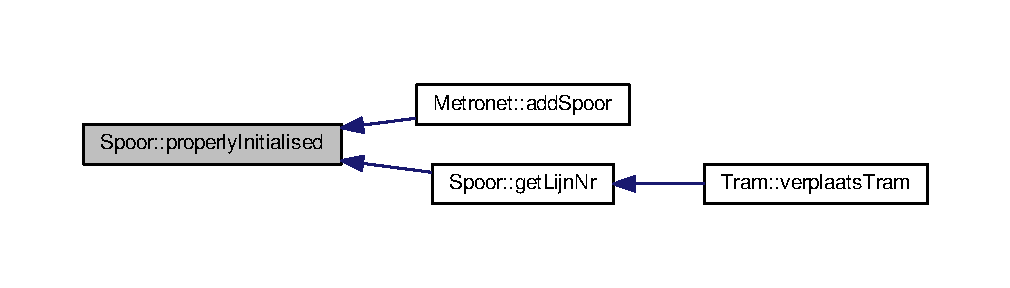
\includegraphics[width=342pt]{class_spoor_a1eb7c54228676cdb7c8620104e063a3c_icgraph}
\end{center}
\end{figure}


The documentation for this class was generated from the following files\+:\begin{DoxyCompactItemize}
\item 
/home/sergio/\+Eclipse\+Projects/\+Soft\+Eng/src/\hyperlink{_spoor_8h}{Spoor.\+h}\item 
/home/sergio/\+Eclipse\+Projects/\+Soft\+Eng/src/\hyperlink{_spoor_8cpp}{Spoor.\+cpp}\end{DoxyCompactItemize}

\hypertarget{class_station}{}\section{Station Class Reference}
\label{class_station}\index{Station@{Station}}


{\ttfamily \#include $<$Station.\+h$>$}

\subsection*{Public Member Functions}
\begin{DoxyCompactItemize}
\item 
\hyperlink{class_station_a73d335726aad1d844d81cda6d9fd74e6}{Station} ()
\item 
\hyperlink{class_station_a1685ff9a628b922fbc6a75f0f23c7b7e}{Station} (std\+::string n, \hyperlink{class_station}{Station} $\ast$vor, \hyperlink{class_station}{Station} $\ast$volg, \hyperlink{class_spoor}{Spoor} $\ast$sp)
\item 
virtual \hyperlink{class_station_a00434e79e8ee7f4ebd6d3b631dde5ac0}{$\sim$\+Station} ()
\item 
bool \hyperlink{class_station_a5749af84d13b71d34aa1fb5b0a935a20}{properly\+Initialised} () const 
\begin{DoxyCompactList}\small\item\em Kijk na of de constructor in de juiste staat geeindigd is. \end{DoxyCompactList}\item 
std\+::string \hyperlink{class_station_a6d4234bcd1027dc83c7984e207e8bd74}{get\+Naam} () const 
\begin{DoxyCompactList}\small\item\em Geef de naam terug van het station. \end{DoxyCompactList}\item 
\hyperlink{class_station}{Station} $\ast$ \hyperlink{class_station_a2adced993339721e8731bfa55762f4f9}{get\+Vorige} () const 
\begin{DoxyCompactList}\small\item\em Geef het vorig station terug. \end{DoxyCompactList}\item 
\hyperlink{class_station}{Station} $\ast$ \hyperlink{class_station_a2c81d14029f13b972c015a16813c8d34}{get\+Volgende} () const 
\begin{DoxyCompactList}\small\item\em Geef het volgende station. \end{DoxyCompactList}\item 
\hyperlink{class_spoor}{Spoor} $\ast$ \hyperlink{class_station_af7ea9d2ec05b56832c0e1a2fe2303ee1}{get\+Spoor} () const 
\begin{DoxyCompactList}\small\item\em Geef het \hyperlink{class_spoor}{Spoor} terug. \end{DoxyCompactList}\end{DoxyCompactItemize}


\subsection{Constructor \& Destructor Documentation}
\index{Station@{Station}!Station@{Station}}
\index{Station@{Station}!Station@{Station}}
\subsubsection[{\texorpdfstring{Station()}{Station()}}]{\setlength{\rightskip}{0pt plus 5cm}Station\+::\+Station (
\begin{DoxyParamCaption}
{}
\end{DoxyParamCaption}
)}\hypertarget{class_station_a73d335726aad1d844d81cda6d9fd74e6}{}\label{class_station_a73d335726aad1d844d81cda6d9fd74e6}
\index{Station@{Station}!Station@{Station}}
\index{Station@{Station}!Station@{Station}}
\subsubsection[{\texorpdfstring{Station(std\+::string n, Station $\ast$vor, Station $\ast$volg, Spoor $\ast$sp)}{Station(std::string n, Station *vor, Station *volg, Spoor *sp)}}]{\setlength{\rightskip}{0pt plus 5cm}Station\+::\+Station (
\begin{DoxyParamCaption}
\item[{std\+::string}]{n, }
\item[{{\bf Station} $\ast$}]{vor, }
\item[{{\bf Station} $\ast$}]{volg, }
\item[{{\bf Spoor} $\ast$}]{sp}
\end{DoxyParamCaption}
)}\hypertarget{class_station_a1685ff9a628b922fbc6a75f0f23c7b7e}{}\label{class_station_a1685ff9a628b922fbc6a75f0f23c7b7e}
\index{Station@{Station}!````~Station@{$\sim$\+Station}}
\index{````~Station@{$\sim$\+Station}!Station@{Station}}
\subsubsection[{\texorpdfstring{$\sim$\+Station()}{~Station()}}]{\setlength{\rightskip}{0pt plus 5cm}Station\+::$\sim$\+Station (
\begin{DoxyParamCaption}
{}
\end{DoxyParamCaption}
)\hspace{0.3cm}{\ttfamily [virtual]}}\hypertarget{class_station_a00434e79e8ee7f4ebd6d3b631dde5ac0}{}\label{class_station_a00434e79e8ee7f4ebd6d3b631dde5ac0}


\subsection{Member Function Documentation}
\index{Station@{Station}!get\+Naam@{get\+Naam}}
\index{get\+Naam@{get\+Naam}!Station@{Station}}
\subsubsection[{\texorpdfstring{get\+Naam() const }{getNaam() const }}]{\setlength{\rightskip}{0pt plus 5cm}std\+::string Station\+::get\+Naam (
\begin{DoxyParamCaption}
{}
\end{DoxyParamCaption}
) const}\hypertarget{class_station_a6d4234bcd1027dc83c7984e207e8bd74}{}\label{class_station_a6d4234bcd1027dc83c7984e207e8bd74}


Geef de naam terug van het station. 

\begin{DoxyReturn}{Returns}
De naam van het station.
\end{DoxyReturn}
R\+E\+Q\+U\+I\+RE(this-\/$>$\hyperlink{class_station_a5749af84d13b71d34aa1fb5b0a935a20}{properly\+Initialised()}, \char`\"{}\+Station was niet geinitialiseerd bij de aanroep van get\+Naam.\char`\"{});~\newline


Here is the call graph for this function\+:
\nopagebreak
\begin{figure}[H]
\begin{center}
\leavevmode
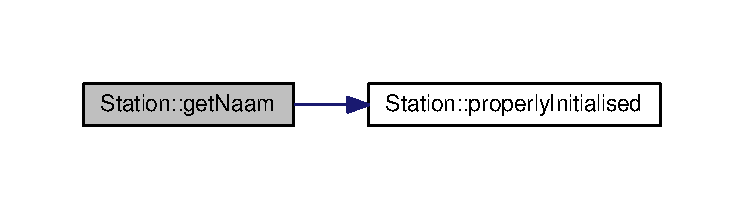
\includegraphics[width=338pt]{class_station_a6d4234bcd1027dc83c7984e207e8bd74_cgraph}
\end{center}
\end{figure}




Here is the caller graph for this function\+:
\nopagebreak
\begin{figure}[H]
\begin{center}
\leavevmode
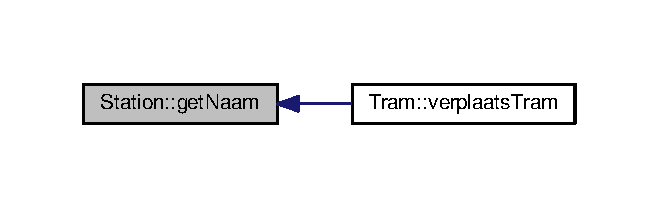
\includegraphics[width=316pt]{class_station_a6d4234bcd1027dc83c7984e207e8bd74_icgraph}
\end{center}
\end{figure}


\index{Station@{Station}!get\+Spoor@{get\+Spoor}}
\index{get\+Spoor@{get\+Spoor}!Station@{Station}}
\subsubsection[{\texorpdfstring{get\+Spoor() const }{getSpoor() const }}]{\setlength{\rightskip}{0pt plus 5cm}{\bf Spoor} $\ast$ Station\+::get\+Spoor (
\begin{DoxyParamCaption}
{}
\end{DoxyParamCaption}
) const}\hypertarget{class_station_af7ea9d2ec05b56832c0e1a2fe2303ee1}{}\label{class_station_af7ea9d2ec05b56832c0e1a2fe2303ee1}


Geef het \hyperlink{class_spoor}{Spoor} terug. 

\begin{DoxyReturn}{Returns}
Het spoor. R\+E\+Q\+U\+I\+RE(this-\/$>$\hyperlink{class_station_a5749af84d13b71d34aa1fb5b0a935a20}{properly\+Initialised()}, \char`\"{}\+Station was niet geinitialiseerd bij de aanroep van get\+Spoor.\char`\"{});~\newline

\end{DoxyReturn}


Here is the call graph for this function\+:
\nopagebreak
\begin{figure}[H]
\begin{center}
\leavevmode
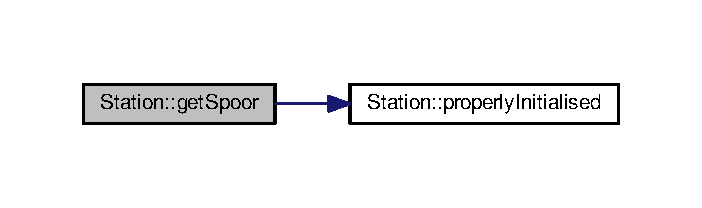
\includegraphics[width=337pt]{class_station_af7ea9d2ec05b56832c0e1a2fe2303ee1_cgraph}
\end{center}
\end{figure}


\index{Station@{Station}!get\+Volgende@{get\+Volgende}}
\index{get\+Volgende@{get\+Volgende}!Station@{Station}}
\subsubsection[{\texorpdfstring{get\+Volgende() const }{getVolgende() const }}]{\setlength{\rightskip}{0pt plus 5cm}{\bf Station} $\ast$ Station\+::get\+Volgende (
\begin{DoxyParamCaption}
{}
\end{DoxyParamCaption}
) const}\hypertarget{class_station_a2c81d14029f13b972c015a16813c8d34}{}\label{class_station_a2c81d14029f13b972c015a16813c8d34}


Geef het volgende station. 

\begin{DoxyReturn}{Returns}
Het volgende station.
\end{DoxyReturn}
R\+E\+Q\+U\+I\+RE(this-\/$>$\hyperlink{class_station_a5749af84d13b71d34aa1fb5b0a935a20}{properly\+Initialised()}, \char`\"{}\+Station was niet geinitialiseerd bij de aanroep van get\+Volgende.\char`\"{});~\newline


Here is the call graph for this function\+:
\nopagebreak
\begin{figure}[H]
\begin{center}
\leavevmode
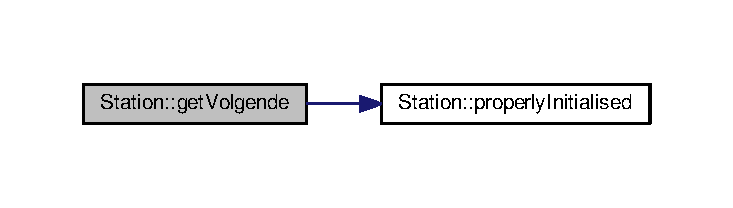
\includegraphics[width=350pt]{class_station_a2c81d14029f13b972c015a16813c8d34_cgraph}
\end{center}
\end{figure}


\index{Station@{Station}!get\+Vorige@{get\+Vorige}}
\index{get\+Vorige@{get\+Vorige}!Station@{Station}}
\subsubsection[{\texorpdfstring{get\+Vorige() const }{getVorige() const }}]{\setlength{\rightskip}{0pt plus 5cm}{\bf Station} $\ast$ Station\+::get\+Vorige (
\begin{DoxyParamCaption}
{}
\end{DoxyParamCaption}
) const}\hypertarget{class_station_a2adced993339721e8731bfa55762f4f9}{}\label{class_station_a2adced993339721e8731bfa55762f4f9}


Geef het vorig station terug. 

\begin{DoxyReturn}{Returns}
Het vorig station.
\end{DoxyReturn}
R\+E\+Q\+U\+I\+RE(this-\/$>$\hyperlink{class_station_a5749af84d13b71d34aa1fb5b0a935a20}{properly\+Initialised()}, \char`\"{}\+Station was niet geinitialiseerd bij de aanroep van get\+Vorige.\char`\"{});~\newline


Here is the call graph for this function\+:
\nopagebreak
\begin{figure}[H]
\begin{center}
\leavevmode
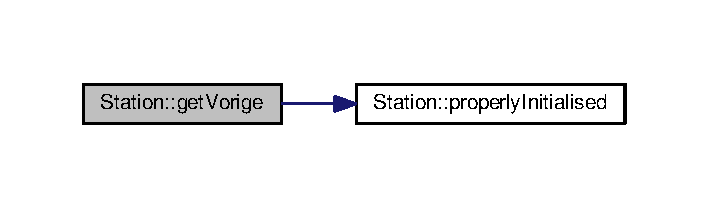
\includegraphics[width=340pt]{class_station_a2adced993339721e8731bfa55762f4f9_cgraph}
\end{center}
\end{figure}


\index{Station@{Station}!properly\+Initialised@{properly\+Initialised}}
\index{properly\+Initialised@{properly\+Initialised}!Station@{Station}}
\subsubsection[{\texorpdfstring{properly\+Initialised() const }{properlyInitialised() const }}]{\setlength{\rightskip}{0pt plus 5cm}bool Station\+::properly\+Initialised (
\begin{DoxyParamCaption}
{}
\end{DoxyParamCaption}
) const}\hypertarget{class_station_a5749af84d13b71d34aa1fb5b0a935a20}{}\label{class_station_a5749af84d13b71d34aa1fb5b0a935a20}


Kijk na of de constructor in de juiste staat geeindigd is. 

\begin{DoxyReturn}{Returns}
Boolean die aangeeft of het object juist geinitialiseerd is. 
\end{DoxyReturn}


Here is the caller graph for this function\+:
\nopagebreak
\begin{figure}[H]
\begin{center}
\leavevmode
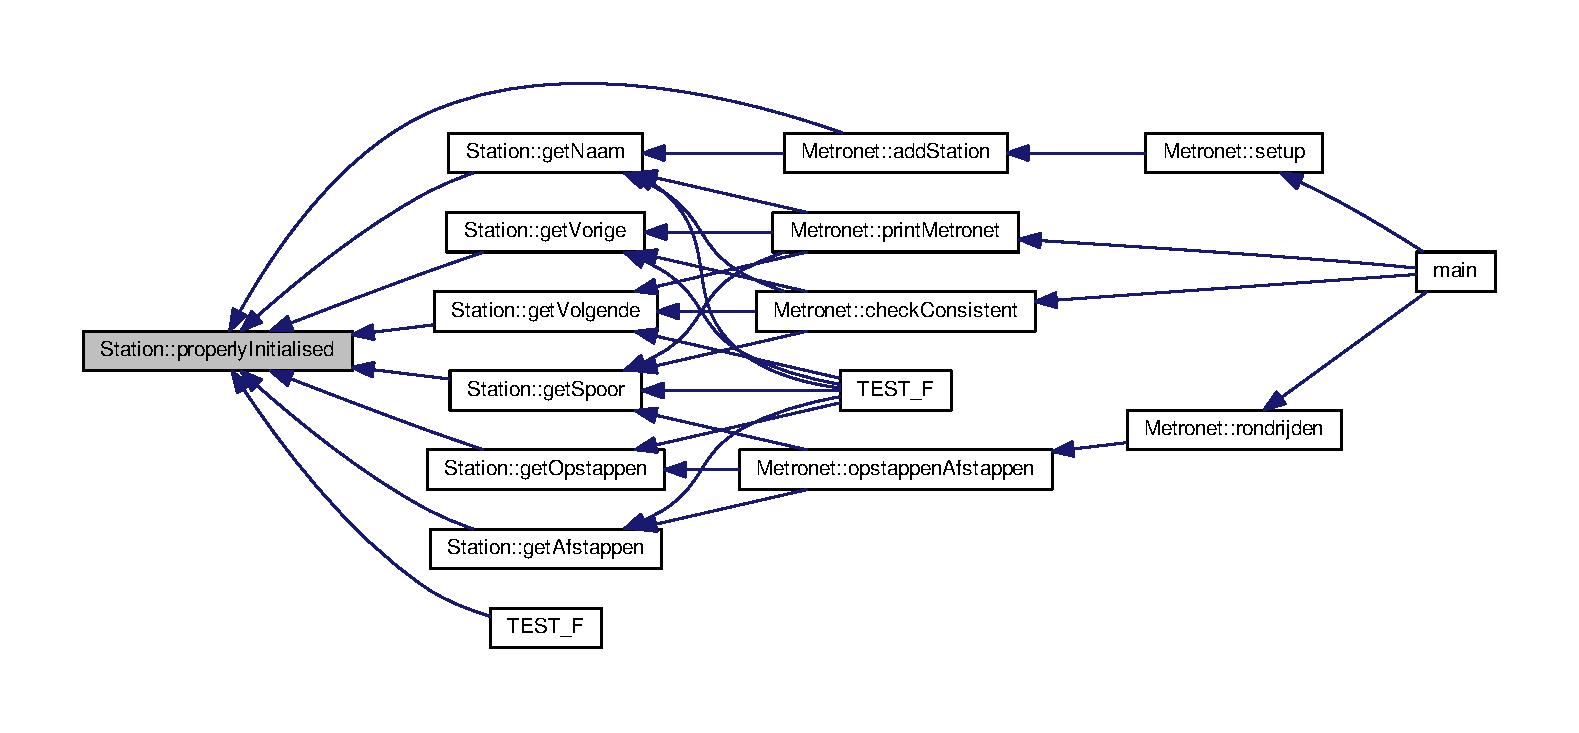
\includegraphics[width=350pt]{class_station_a5749af84d13b71d34aa1fb5b0a935a20_icgraph}
\end{center}
\end{figure}




The documentation for this class was generated from the following files\+:\begin{DoxyCompactItemize}
\item 
/home/jonathan/\+Desktop/\+Project Software Engineering/\+Metronet/\+P\+S\+E/src/\hyperlink{_station_8h}{Station.\+h}\item 
/home/jonathan/\+Desktop/\+Project Software Engineering/\+Metronet/\+P\+S\+E/src/\hyperlink{_station_8cpp}{Station.\+cpp}\end{DoxyCompactItemize}

\hypertarget{class_tram}{}\section{Tram Class Reference}
\label{class_tram}\index{Tram@{Tram}}


{\ttfamily \#include $<$Tram.\+h$>$}

\subsection*{Public Member Functions}
\begin{DoxyCompactItemize}
\item 
\hyperlink{class_tram_aad83b2e7e79d57528691bf317ab0e1ef}{Tram} ()
\item 
\hyperlink{class_tram_afef6559a85225dc0b8a9445d6d16cbbb}{Tram} (int zit, int snel, int sp, std\+::string beginS)
\item 
bool \hyperlink{class_tram_a98992eff0453f54fbe64e1f1064169c7}{properly\+Initialised} () const 
\begin{DoxyCompactList}\small\item\em Kijk na of de constructor in de juiste staat geeindigd is. \end{DoxyCompactList}\item 
int \hyperlink{class_tram_aa366e37291186d6cfd402aa7b6cfec2d}{get\+Zitplaatsen} () const 
\begin{DoxyCompactList}\small\item\em Geef de zitplaatsen terug van de tram. \end{DoxyCompactList}\item 
int \hyperlink{class_tram_a8e9e449f0032f0f439c196e0980a891e}{get\+Passagiers} () const 
\begin{DoxyCompactList}\small\item\em Geef de passagiers terug van de tram. \end{DoxyCompactList}\item 
int \hyperlink{class_tram_a40a12ae66cdc8965fc73d548dd038e4c}{get\+Snelheid} () const 
\begin{DoxyCompactList}\small\item\em Geef de snelheid terug van de tram. \end{DoxyCompactList}\item 
int \hyperlink{class_tram_a52655f991ffb58a8ab3557fd881a6f58}{get\+Spoor} () const 
\begin{DoxyCompactList}\small\item\em Geef het spoor terug. \end{DoxyCompactList}\item 
std\+::string \hyperlink{class_tram_aba7b84414cd60d013ac1db3f3403497d}{get\+Begin\+Station} () const 
\begin{DoxyCompactList}\small\item\em Geef het beginstation terug. \end{DoxyCompactList}\item 
std\+::string \hyperlink{class_tram_ae7bc337a42b2d839b4da5f648b781e79}{get\+Huidig\+Station} () const 
\begin{DoxyCompactList}\small\item\em Geef het huidig station. \end{DoxyCompactList}\item 
void \hyperlink{class_tram_a8d55296c7ede4aa92c9b3a4b2a9495a8}{verplaats\+Tram} (std\+::string station, \hyperlink{class_exporter}{Exporter} $\ast$exp, std\+::ostream \&os)
\begin{DoxyCompactList}\small\item\em Verplaatst een tram naar het opgegeven station. \end{DoxyCompactList}\item 
bool \hyperlink{class_tram_a81186910caa5212b4a87eec84cd10a46}{afstappen} (int afstappen)
\begin{DoxyCompactList}\small\item\em Emuleert afstappen van passagiers. (Nieuw huidig aantal = huidig aantal -\/ afstappende passagiers) \end{DoxyCompactList}\item 
bool \hyperlink{class_tram_aaeb00c535a6854f85dcc42cdff97ad0c}{opstappen} (int opstappen)
\begin{DoxyCompactList}\small\item\em Emuleert opstappen van passagiers. (Nieuw huidig aantal = huidig aantal + opstappende passagiers) \end{DoxyCompactList}\end{DoxyCompactItemize}


\subsection{Constructor \& Destructor Documentation}
\index{Tram@{Tram}!Tram@{Tram}}
\index{Tram@{Tram}!Tram@{Tram}}
\subsubsection[{\texorpdfstring{Tram()}{Tram()}}]{\setlength{\rightskip}{0pt plus 5cm}Tram\+::\+Tram (
\begin{DoxyParamCaption}
{}
\end{DoxyParamCaption}
)}\hypertarget{class_tram_aad83b2e7e79d57528691bf317ab0e1ef}{}\label{class_tram_aad83b2e7e79d57528691bf317ab0e1ef}
\index{Tram@{Tram}!Tram@{Tram}}
\index{Tram@{Tram}!Tram@{Tram}}
\subsubsection[{\texorpdfstring{Tram(int zit, int snel, int sp, std\+::string begin\+S)}{Tram(int zit, int snel, int sp, std::string beginS)}}]{\setlength{\rightskip}{0pt plus 5cm}Tram\+::\+Tram (
\begin{DoxyParamCaption}
\item[{int}]{zit, }
\item[{int}]{snel, }
\item[{int}]{sp, }
\item[{std\+::string}]{beginS}
\end{DoxyParamCaption}
)}\hypertarget{class_tram_afef6559a85225dc0b8a9445d6d16cbbb}{}\label{class_tram_afef6559a85225dc0b8a9445d6d16cbbb}


\subsection{Member Function Documentation}
\index{Tram@{Tram}!afstappen@{afstappen}}
\index{afstappen@{afstappen}!Tram@{Tram}}
\subsubsection[{\texorpdfstring{afstappen(int afstappen)}{afstappen(int afstappen)}}]{\setlength{\rightskip}{0pt plus 5cm}bool Tram\+::afstappen (
\begin{DoxyParamCaption}
\item[{int}]{afstappen}
\end{DoxyParamCaption}
)}\hypertarget{class_tram_a81186910caa5212b4a87eec84cd10a46}{}\label{class_tram_a81186910caa5212b4a87eec84cd10a46}


Emuleert afstappen van passagiers. (Nieuw huidig aantal = huidig aantal -\/ afstappende passagiers) 


\begin{DoxyParams}{Parameters}
{\em afstappen} & Aantal passagiers dat afstapt. \\
\hline
\end{DoxyParams}
\begin{DoxyReturn}{Returns}
boolean Of er meer passagiers afstapten dan mogelijk.
\end{DoxyReturn}
R\+E\+Q\+U\+I\+RE(this-\/$>$\hyperlink{class_tram_a98992eff0453f54fbe64e1f1064169c7}{properly\+Initialised()}, \char`\"{}\+Tram was niet geinitialiseerd bij de aanroep van afstappen.\char`\"{});~\newline


Here is the call graph for this function\+:
\nopagebreak
\begin{figure}[H]
\begin{center}
\leavevmode
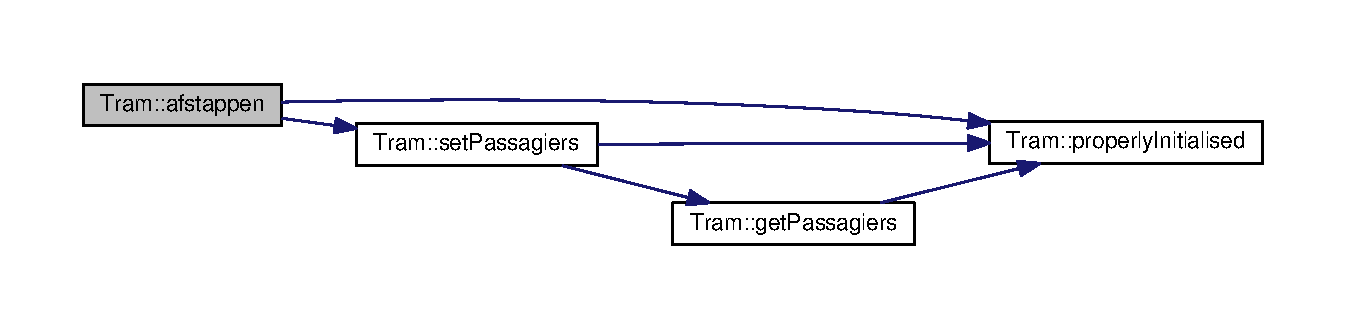
\includegraphics[width=325pt]{class_tram_a81186910caa5212b4a87eec84cd10a46_cgraph}
\end{center}
\end{figure}




Here is the caller graph for this function\+:
\nopagebreak
\begin{figure}[H]
\begin{center}
\leavevmode
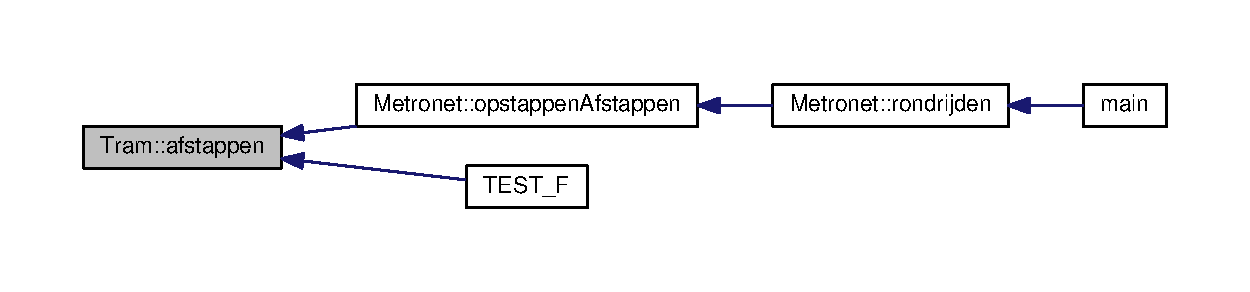
\includegraphics[width=350pt]{class_tram_a81186910caa5212b4a87eec84cd10a46_icgraph}
\end{center}
\end{figure}


\index{Tram@{Tram}!get\+Begin\+Station@{get\+Begin\+Station}}
\index{get\+Begin\+Station@{get\+Begin\+Station}!Tram@{Tram}}
\subsubsection[{\texorpdfstring{get\+Begin\+Station() const }{getBeginStation() const }}]{\setlength{\rightskip}{0pt plus 5cm}std\+::string Tram\+::get\+Begin\+Station (
\begin{DoxyParamCaption}
{}
\end{DoxyParamCaption}
) const}\hypertarget{class_tram_aba7b84414cd60d013ac1db3f3403497d}{}\label{class_tram_aba7b84414cd60d013ac1db3f3403497d}


Geef het beginstation terug. 

\begin{DoxyReturn}{Returns}
Het beginstation.
\end{DoxyReturn}
R\+E\+Q\+U\+I\+RE(this-\/$>$\hyperlink{class_tram_a98992eff0453f54fbe64e1f1064169c7}{properly\+Initialised()}, \char`\"{}\+Tram was niet geinitialiseerd bij de aanroep van get\+Begin\+Station.\char`\"{});~\newline


Here is the call graph for this function\+:
\nopagebreak
\begin{figure}[H]
\begin{center}
\leavevmode
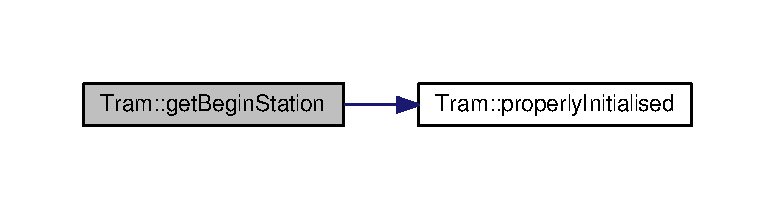
\includegraphics[width=350pt]{class_tram_aba7b84414cd60d013ac1db3f3403497d_cgraph}
\end{center}
\end{figure}




Here is the caller graph for this function\+:
\nopagebreak
\begin{figure}[H]
\begin{center}
\leavevmode
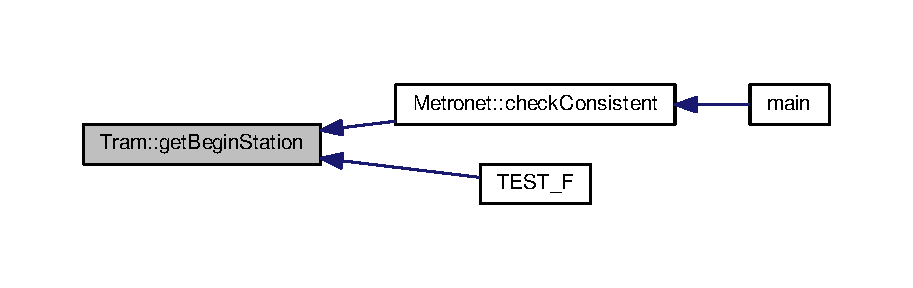
\includegraphics[width=350pt]{class_tram_aba7b84414cd60d013ac1db3f3403497d_icgraph}
\end{center}
\end{figure}


\index{Tram@{Tram}!get\+Huidig\+Station@{get\+Huidig\+Station}}
\index{get\+Huidig\+Station@{get\+Huidig\+Station}!Tram@{Tram}}
\subsubsection[{\texorpdfstring{get\+Huidig\+Station() const }{getHuidigStation() const }}]{\setlength{\rightskip}{0pt plus 5cm}std\+::string Tram\+::get\+Huidig\+Station (
\begin{DoxyParamCaption}
{}
\end{DoxyParamCaption}
) const}\hypertarget{class_tram_ae7bc337a42b2d839b4da5f648b781e79}{}\label{class_tram_ae7bc337a42b2d839b4da5f648b781e79}


Geef het huidig station. 

\begin{DoxyReturn}{Returns}
Het huidig station.
\end{DoxyReturn}
R\+E\+Q\+U\+I\+RE(this-\/$>$\hyperlink{class_tram_a98992eff0453f54fbe64e1f1064169c7}{properly\+Initialised()}, \char`\"{}\+Tram was niet geinitialiseerd bij de aanroep van get\+Huidig\+Station.\char`\"{});~\newline


Here is the call graph for this function\+:
\nopagebreak
\begin{figure}[H]
\begin{center}
\leavevmode
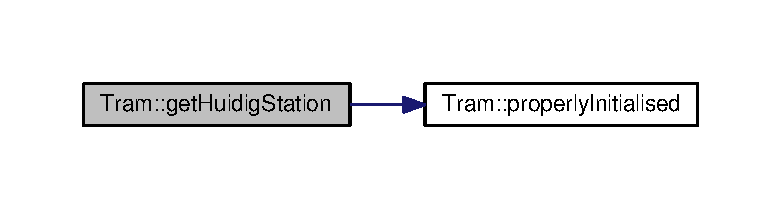
\includegraphics[width=350pt]{class_tram_ae7bc337a42b2d839b4da5f648b781e79_cgraph}
\end{center}
\end{figure}




Here is the caller graph for this function\+:
\nopagebreak
\begin{figure}[H]
\begin{center}
\leavevmode
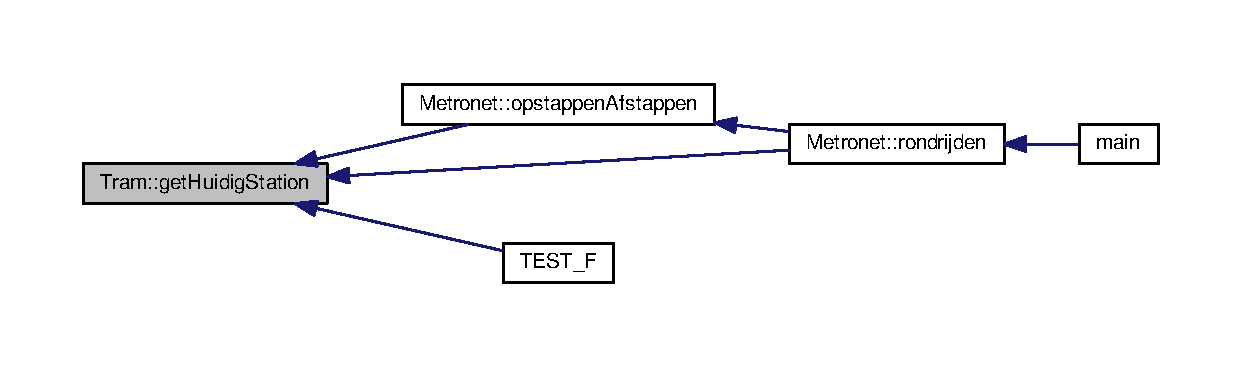
\includegraphics[width=350pt]{class_tram_ae7bc337a42b2d839b4da5f648b781e79_icgraph}
\end{center}
\end{figure}


\index{Tram@{Tram}!get\+Passagiers@{get\+Passagiers}}
\index{get\+Passagiers@{get\+Passagiers}!Tram@{Tram}}
\subsubsection[{\texorpdfstring{get\+Passagiers() const }{getPassagiers() const }}]{\setlength{\rightskip}{0pt plus 5cm}int Tram\+::get\+Passagiers (
\begin{DoxyParamCaption}
{}
\end{DoxyParamCaption}
) const}\hypertarget{class_tram_a8e9e449f0032f0f439c196e0980a891e}{}\label{class_tram_a8e9e449f0032f0f439c196e0980a891e}


Geef de passagiers terug van de tram. 

\begin{DoxyReturn}{Returns}
De passagiers.
\end{DoxyReturn}
R\+E\+Q\+U\+I\+RE(this-\/$>$\hyperlink{class_tram_a98992eff0453f54fbe64e1f1064169c7}{properly\+Initialised()}, \char`\"{}\+Tram was niet geinitialiseerd bij de aanroep van get\+Passagiers.\char`\"{});~\newline


Here is the call graph for this function\+:\nopagebreak
\begin{figure}[H]
\begin{center}
\leavevmode
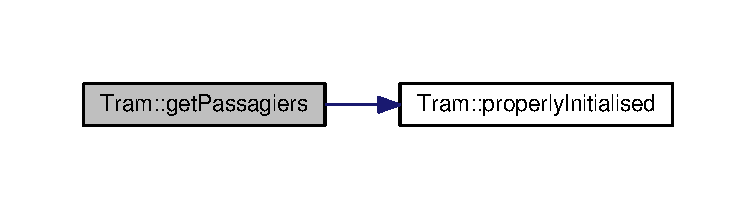
\includegraphics[width=344pt]{class_tram_a8e9e449f0032f0f439c196e0980a891e_cgraph}
\end{center}
\end{figure}


\index{Tram@{Tram}!get\+Snelheid@{get\+Snelheid}}
\index{get\+Snelheid@{get\+Snelheid}!Tram@{Tram}}
\subsubsection[{\texorpdfstring{get\+Snelheid() const }{getSnelheid() const }}]{\setlength{\rightskip}{0pt plus 5cm}int Tram\+::get\+Snelheid (
\begin{DoxyParamCaption}
{}
\end{DoxyParamCaption}
) const}\hypertarget{class_tram_a40a12ae66cdc8965fc73d548dd038e4c}{}\label{class_tram_a40a12ae66cdc8965fc73d548dd038e4c}


Geef de snelheid terug van de tram. 

\begin{DoxyReturn}{Returns}
De snelheid.
\end{DoxyReturn}
R\+E\+Q\+U\+I\+RE(this-\/$>$\hyperlink{class_tram_a98992eff0453f54fbe64e1f1064169c7}{properly\+Initialised()}, \char`\"{}\+Tram was niet geinitialiseerd bij de aanroep van get\+Snelheid.\char`\"{});~\newline


Here is the call graph for this function\+:\nopagebreak
\begin{figure}[H]
\begin{center}
\leavevmode
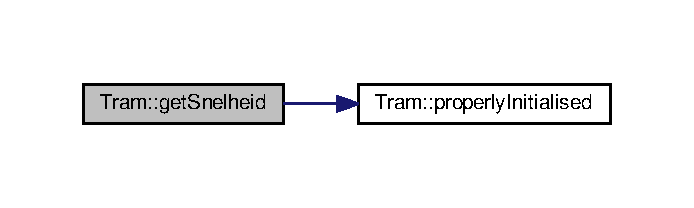
\includegraphics[width=333pt]{class_tram_a40a12ae66cdc8965fc73d548dd038e4c_cgraph}
\end{center}
\end{figure}


\index{Tram@{Tram}!get\+Spoor@{get\+Spoor}}
\index{get\+Spoor@{get\+Spoor}!Tram@{Tram}}
\subsubsection[{\texorpdfstring{get\+Spoor() const }{getSpoor() const }}]{\setlength{\rightskip}{0pt plus 5cm}int Tram\+::get\+Spoor (
\begin{DoxyParamCaption}
{}
\end{DoxyParamCaption}
) const}\hypertarget{class_tram_a52655f991ffb58a8ab3557fd881a6f58}{}\label{class_tram_a52655f991ffb58a8ab3557fd881a6f58}


Geef het spoor terug. 

\begin{DoxyReturn}{Returns}
Het spoor.
\end{DoxyReturn}
R\+E\+Q\+U\+I\+RE(this-\/$>$\hyperlink{class_tram_a98992eff0453f54fbe64e1f1064169c7}{properly\+Initialised()}, \char`\"{}\+Tram was niet geinitialiseerd bij de aanroep van get\+Spoor.\char`\"{});~\newline


Here is the call graph for this function\+:
\nopagebreak
\begin{figure}[H]
\begin{center}
\leavevmode
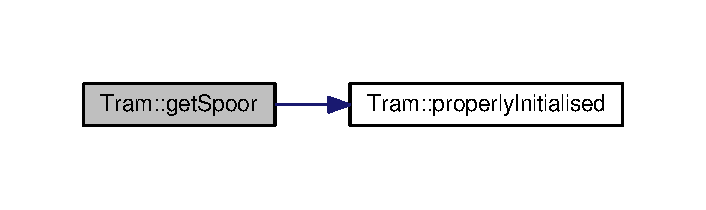
\includegraphics[width=321pt]{class_tram_a52655f991ffb58a8ab3557fd881a6f58_cgraph}
\end{center}
\end{figure}




Here is the caller graph for this function\+:
\nopagebreak
\begin{figure}[H]
\begin{center}
\leavevmode
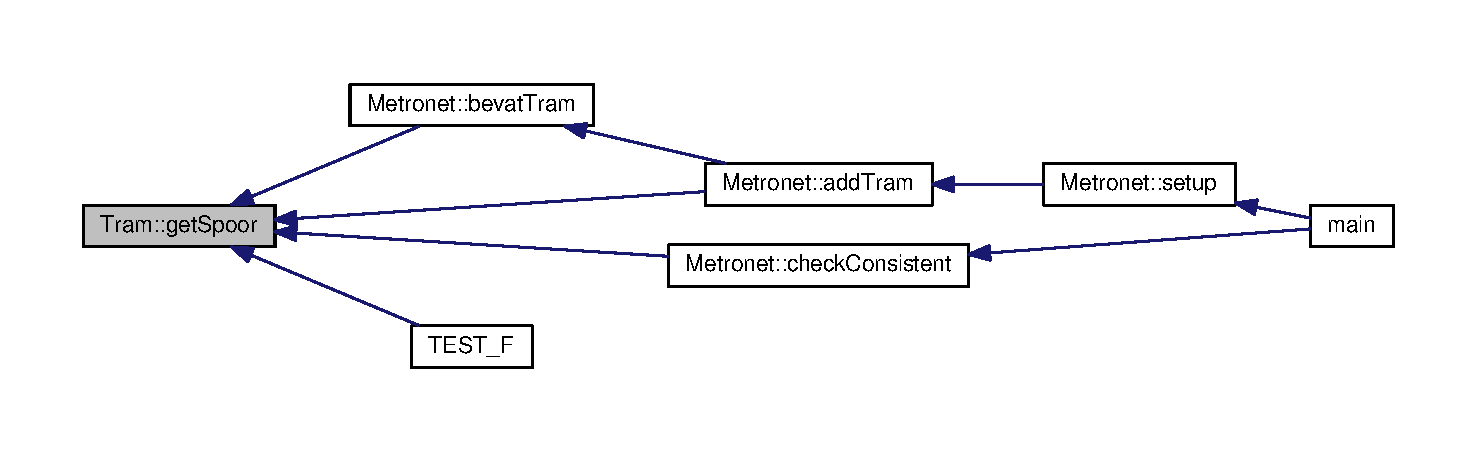
\includegraphics[width=350pt]{class_tram_a52655f991ffb58a8ab3557fd881a6f58_icgraph}
\end{center}
\end{figure}


\index{Tram@{Tram}!get\+Zitplaatsen@{get\+Zitplaatsen}}
\index{get\+Zitplaatsen@{get\+Zitplaatsen}!Tram@{Tram}}
\subsubsection[{\texorpdfstring{get\+Zitplaatsen() const }{getZitplaatsen() const }}]{\setlength{\rightskip}{0pt plus 5cm}int Tram\+::get\+Zitplaatsen (
\begin{DoxyParamCaption}
{}
\end{DoxyParamCaption}
) const}\hypertarget{class_tram_aa366e37291186d6cfd402aa7b6cfec2d}{}\label{class_tram_aa366e37291186d6cfd402aa7b6cfec2d}


Geef de zitplaatsen terug van de tram. 

\begin{DoxyReturn}{Returns}
De zitplaatsen.
\end{DoxyReturn}
R\+E\+Q\+U\+I\+RE(this-\/$>$\hyperlink{class_tram_a98992eff0453f54fbe64e1f1064169c7}{properly\+Initialised()}, \char`\"{}\+Tram was niet geinitialiseerd bij de aanroep van get\+Zitplaatsen.\char`\"{});~\newline


Here is the call graph for this function\+:\nopagebreak
\begin{figure}[H]
\begin{center}
\leavevmode
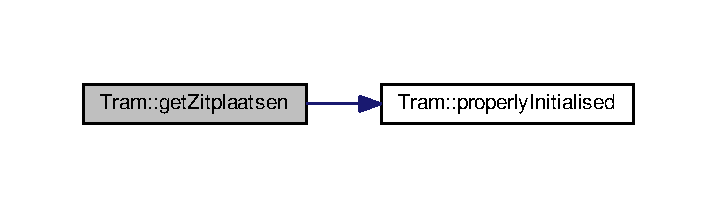
\includegraphics[width=344pt]{class_tram_aa366e37291186d6cfd402aa7b6cfec2d_cgraph}
\end{center}
\end{figure}


\index{Tram@{Tram}!opstappen@{opstappen}}
\index{opstappen@{opstappen}!Tram@{Tram}}
\subsubsection[{\texorpdfstring{opstappen(int opstappen)}{opstappen(int opstappen)}}]{\setlength{\rightskip}{0pt plus 5cm}bool Tram\+::opstappen (
\begin{DoxyParamCaption}
\item[{int}]{opstappen}
\end{DoxyParamCaption}
)}\hypertarget{class_tram_aaeb00c535a6854f85dcc42cdff97ad0c}{}\label{class_tram_aaeb00c535a6854f85dcc42cdff97ad0c}


Emuleert opstappen van passagiers. (Nieuw huidig aantal = huidig aantal + opstappende passagiers) 


\begin{DoxyParams}{Parameters}
{\em opstappen} & Aantal passagiers dat opstapt. \\
\hline
\end{DoxyParams}
\begin{DoxyReturn}{Returns}
boolean Of er meer passigiers opstapten dan mogelijk.
\end{DoxyReturn}
R\+E\+Q\+U\+I\+RE(this-\/$>$\hyperlink{class_tram_a98992eff0453f54fbe64e1f1064169c7}{properly\+Initialised()}, \char`\"{}\+Tram was niet geinitialiseerd bij de aanroep van opstappen.\char`\"{});~\newline


Here is the call graph for this function\+:
\nopagebreak
\begin{figure}[H]
\begin{center}
\leavevmode
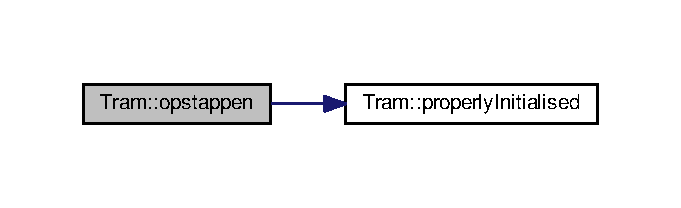
\includegraphics[width=327pt]{class_tram_aaeb00c535a6854f85dcc42cdff97ad0c_cgraph}
\end{center}
\end{figure}




Here is the caller graph for this function\+:
\nopagebreak
\begin{figure}[H]
\begin{center}
\leavevmode
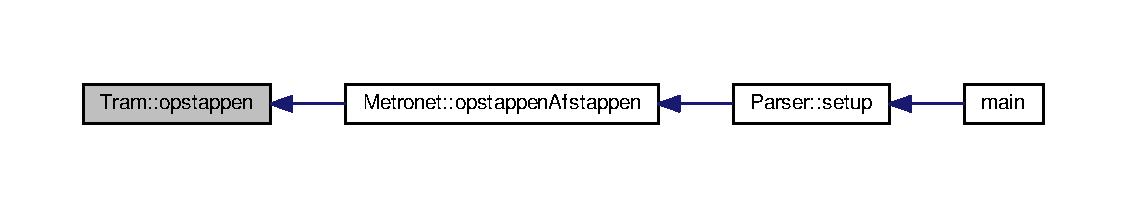
\includegraphics[width=350pt]{class_tram_aaeb00c535a6854f85dcc42cdff97ad0c_icgraph}
\end{center}
\end{figure}


\index{Tram@{Tram}!properly\+Initialised@{properly\+Initialised}}
\index{properly\+Initialised@{properly\+Initialised}!Tram@{Tram}}
\subsubsection[{\texorpdfstring{properly\+Initialised() const }{properlyInitialised() const }}]{\setlength{\rightskip}{0pt plus 5cm}bool Tram\+::properly\+Initialised (
\begin{DoxyParamCaption}
{}
\end{DoxyParamCaption}
) const}\hypertarget{class_tram_a98992eff0453f54fbe64e1f1064169c7}{}\label{class_tram_a98992eff0453f54fbe64e1f1064169c7}


Kijk na of de constructor in de juiste staat geeindigd is. 

\begin{DoxyReturn}{Returns}
Boolean die aangeeft of het object juist geinitialiseerd is. 
\end{DoxyReturn}


Here is the caller graph for this function\+:
\nopagebreak
\begin{figure}[H]
\begin{center}
\leavevmode
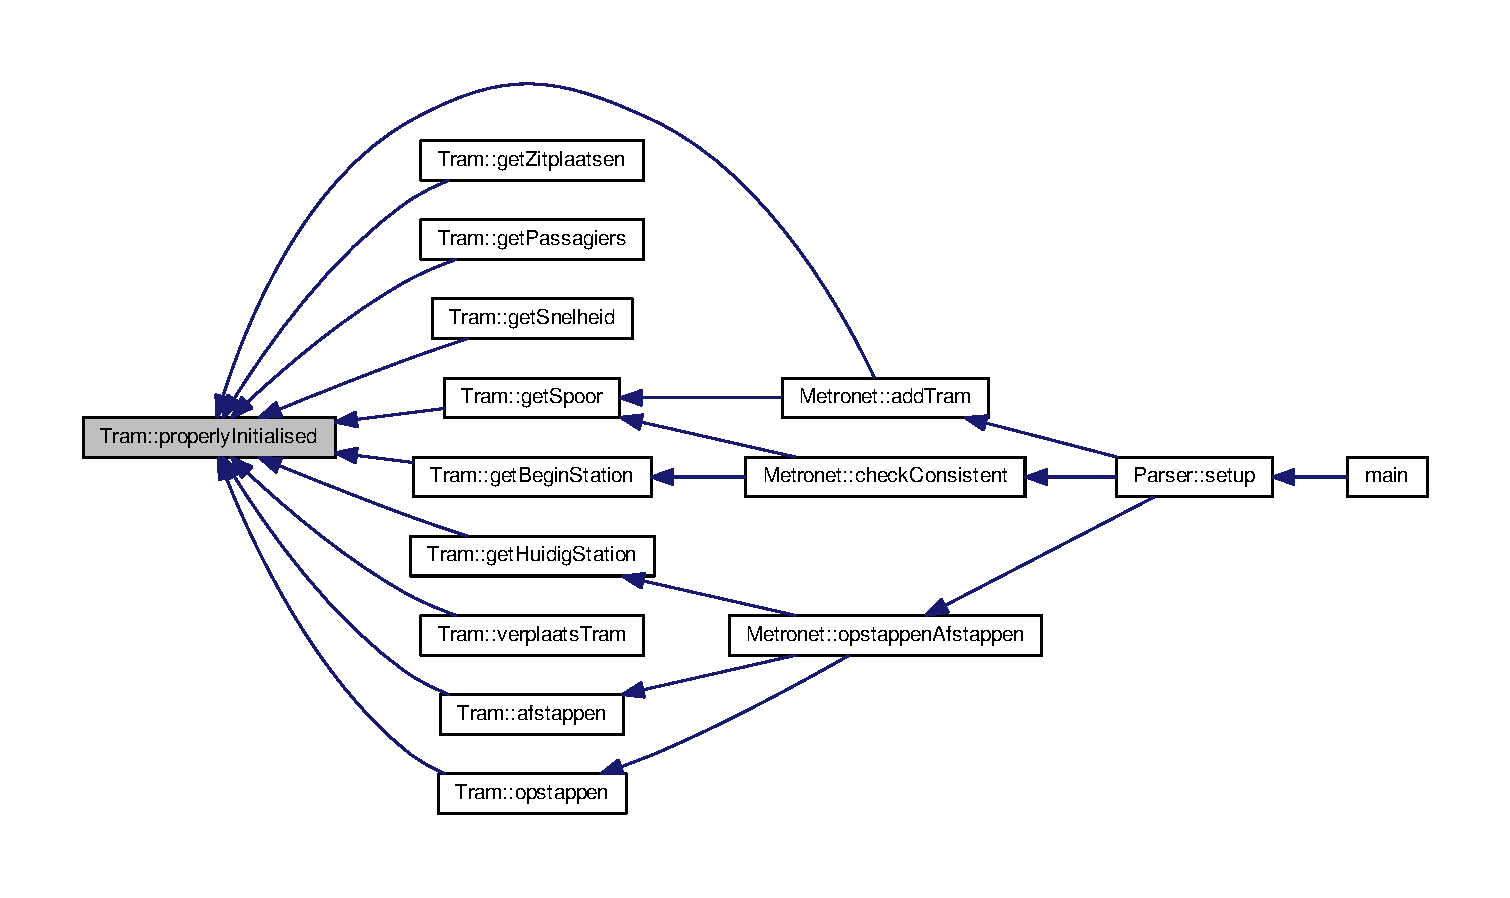
\includegraphics[width=350pt]{class_tram_a98992eff0453f54fbe64e1f1064169c7_icgraph}
\end{center}
\end{figure}


\index{Tram@{Tram}!verplaats\+Tram@{verplaats\+Tram}}
\index{verplaats\+Tram@{verplaats\+Tram}!Tram@{Tram}}
\subsubsection[{\texorpdfstring{verplaats\+Tram(std\+::string station, Exporter $\ast$exp, std\+::ostream \&os)}{verplaatsTram(std::string station, Exporter *exp, std::ostream &os)}}]{\setlength{\rightskip}{0pt plus 5cm}void Tram\+::verplaats\+Tram (
\begin{DoxyParamCaption}
\item[{std\+::string}]{station, }
\item[{{\bf Exporter} $\ast$}]{exp, }
\item[{std\+::ostream \&}]{os}
\end{DoxyParamCaption}
)}\hypertarget{class_tram_a8d55296c7ede4aa92c9b3a4b2a9495a8}{}\label{class_tram_a8d55296c7ede4aa92c9b3a4b2a9495a8}


Verplaatst een tram naar het opgegeven station. 

R\+E\+Q\+U\+I\+RE(this-\/$>$\hyperlink{class_tram_a98992eff0453f54fbe64e1f1064169c7}{properly\+Initialised()}, \char`\"{}\+Tram was niet geinitialiseerd bij de aanroep van verplaats\+Tram.\char`\"{});~\newline
E\+N\+S\+U\+RE((huidig\+Station == station), \char`\"{}huidig\+Station is niet correct aangepast.\char`\"{});~\newline


Here is the call graph for this function\+:
\nopagebreak
\begin{figure}[H]
\begin{center}
\leavevmode
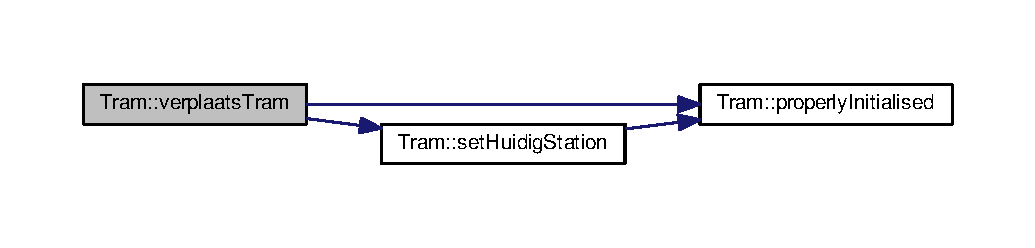
\includegraphics[width=344pt]{class_tram_a8d55296c7ede4aa92c9b3a4b2a9495a8_cgraph}
\end{center}
\end{figure}




The documentation for this class was generated from the following files\+:\begin{DoxyCompactItemize}
\item 
/home/jonathan/\+Desktop/\+Project Software Engineering/\+Metronet/\+P\+S\+E/src/\hyperlink{_tram_8h}{Tram.\+h}\item 
/home/jonathan/\+Desktop/\+Project Software Engineering/\+Metronet/\+P\+S\+E/src/\hyperlink{_tram_8cpp}{Tram.\+cpp}\end{DoxyCompactItemize}

%--- End generated contents ---

% Index
\backmatter
\newpage
\phantomsection
\clearemptydoublepage
\addcontentsline{toc}{chapter}{Index}
\printindex

\end{document}
